\documentclass{article}
\usepackage{float}
\usepackage[utf8]{vietnam} % Hỗ trợ tiếng Việt
\usepackage{graphicx} % Để chèn hình ảnh
\usepackage{amsmath} % Để viết công thức toán học
\usepackage{hyperref} % Để tạo mục lục liên kết
\usepackage{subcaption} % Để tạo subfigure
\usepackage{array} % Để hỗ trợ bảng
\usepackage[left=1.00in, right=1.00in, top=1.00in, bottom=1.00in]{geometry} % Điều chỉnh lề

% Tiêu đề tài liệu
\begin{document}

% Trang bìa
\begin{center}
    \textbf{TRƯỜNG ĐẠI HỌC XÂY DỰNG HÀ NỘI} \\
    \vspace{0.5cm}
    \textbf{KHOA CÔNG NGHỆ THÔNG TIN} \\
    \vspace{0.5cm}
    
\includegraphics[width=0.5\textwidth]{image1.png} \\
    \vspace{0.5cm}
    \textbf{BÁO CÁO MÔN HỌC: NHẬN DIỆN CÓ ĐỘI MŨ BẢO HIỂM VỚI FASTER-RCNN} \\
    \vspace{1cm}
    \begin{tabular}{ll}
        \textbf{GVHD:} & Nguyễn Đình Quý \\
        \textbf{Nhóm:} & 6 \\
        \textbf{Thành viên:} & 0338967 – Nguyễn Quang Minh \\
        & 0212267 – Lâm Quang Huy \\
        & 0117967 – Trần Nhật Minh \\
        & 0016967 – Tống Thiên Bảo \\
    \end{tabular} \\
    \vspace{1cm}
    Hà Nội, Năm 2025
\end{center}

\newpage

% Mục lục
\tableofcontents
\newpage

% Phần 1: Faster R-CNN
\section{Faster R-CNN}
Faster R-CNN (Faster Region-Convolutional Neural Network) là một kiến trúc mạng nơ-ron tích chập sâu (CNN) hiện đại được sử dụng cho nhiệm vụ phát hiện đối tượng trong ảnh, cải thiện đáng kể tốc độ và độ chính xác so với các phiên bản trước đó như R-CNN và Fast R-CNN.

\begin{figure}[H]
    \centering
    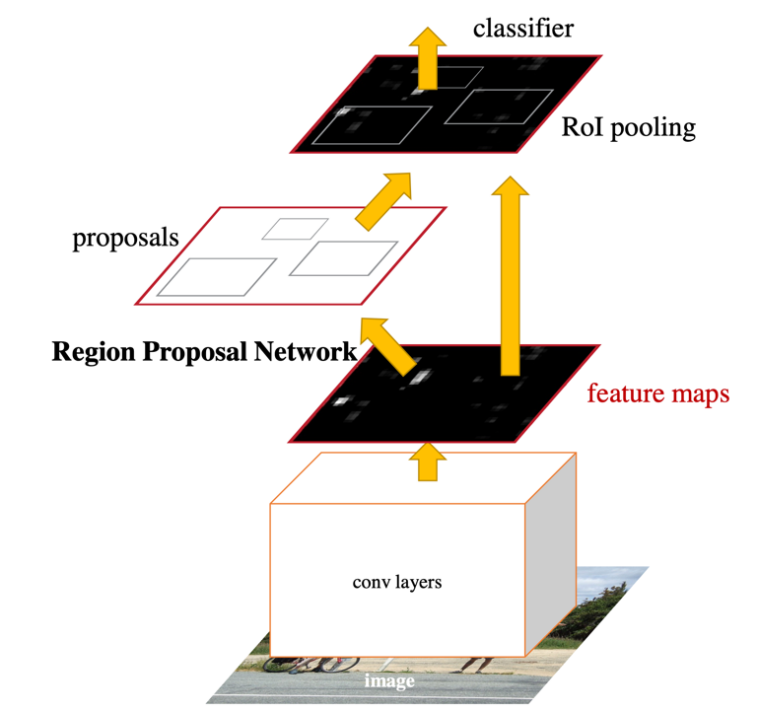
\includegraphics[width=0.8\textwidth]{image2.png}
    \caption{Mô hình Faster R-CNN}
\end{figure}

\begin{itemize}
    \item Thay vì cho ảnh vào trực tiếp sử dụng thuật toán Selective Search như các mô hình trước đây như R-CNN, Fast R-CNN, thì Faster R-CNN dùng một mạng RPN (Region Proposal Network) để trích xuất ra các vùng có khả năng chứa đối tượng, về cơ bản thì nó cải thiện được tốc độ hơn rất nhiều.
    \item Mô hình của Faster R-CNN sẽ chính xác hơn do sử dụng mô hình CNN mạnh như ResNet hoặc VGG16 để trích xuất đặc trưng.
    \item Một trong những cải tiến quan trọng của Faster R-CNN là việc chia sẻ các lớp tích chập giữa RPN và Fast R-CNN, nghĩa là cả hai mô-đun đều hoạt động trên cùng một feature map được tính toán một lần, giúp giảm đáng kể chi phí tính toán và tăng tốc độ.
    \item Mô hình Faster R-CNN có thể dự đoán được đối tượng dựa trên thời gian thực trên GPU.
    \item Một số nhược điểm:
    \begin{itemize}
        \item Mô hình nặng do sử dụng nhiều mô hình (ví dụ VGG, ResNet) sẽ không thể dùng trên các thiết bị yếu.
        \item Faster R-CNN thường hoạt động không tốt với các vật thể nhỏ hoặc vật thể có kích thước thay đổi lớn trong cùng một ảnh.
    \end{itemize}
\end{itemize}

% Phần 2: Kiến trúc của Faster R-CNN
\section{Kiến trúc của Faster R-CNN}
\begin{figure}[H]
    \centering
    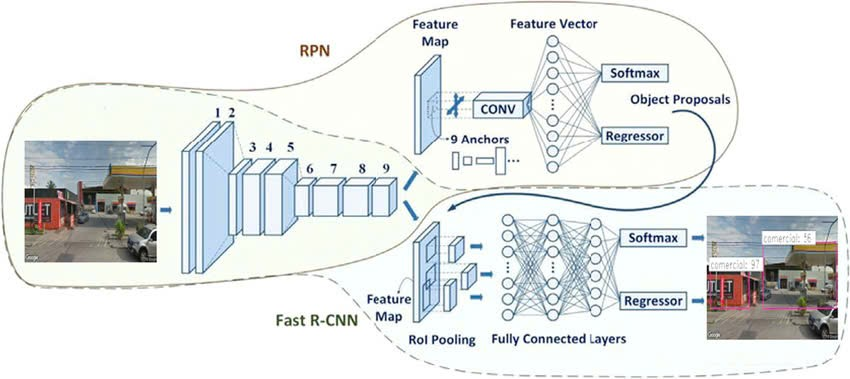
\includegraphics[width=0.8\textwidth]{image3.png}
    \caption{Kiến trúc của Faster R-CNN}
\end{figure}

\subsection{Trích xuất đặc trưng}
Dùng mạng CNN sâu như VGG16, ResNet-50, ResNet-101 để tạo Feature Map từ ảnh đầu vào.

\begin{figure}[H]
    \centering
    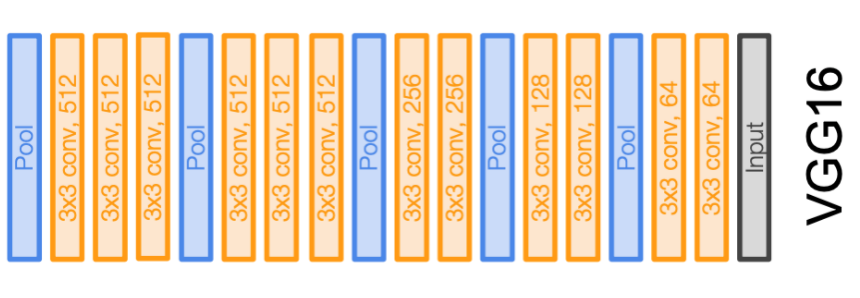
\includegraphics[width=0.8\textwidth]{image4.png}
    \caption{Ví dụ Feature Map}
\end{figure}

Các lớp Conv trong backbone giúp trích xuất các đặc trưng quan trọng như cạnh, góc, texture. \\
Output: Feature Map, dùng làm đầu vào cho RPN. Ví dụ, ảnh có kích thước 1024x1024 khi đi qua ResNet-50 sẽ cho kích thước của feature map là 64x64, giúp giảm kích thước và tăng tốc độ xử lý.

\subsection{Anchors}
Là một bước trong RPN có tác dụng đề xuất các anchor box tại mỗi điểm của feature map. \\
Số hộp sẽ là $k$, trong cấu hình mặc định của Faster R-CNN sẽ là 9.

\begin{figure}[H]
    \begin{subfigure}{0.45\textwidth}
        \centering
        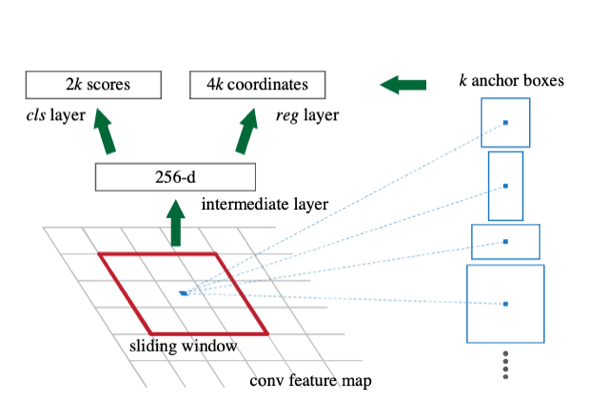
\includegraphics[width=\textwidth]{image5.png}
    \end{subfigure}
    \hfill
    \begin{subfigure}{0.45\textwidth}
        \centering
        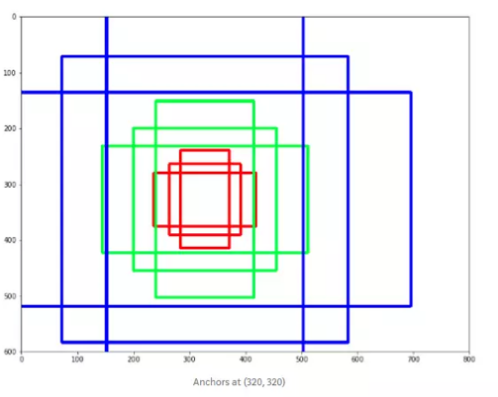
\includegraphics[width=\textwidth]{image6.png}
    \end{subfigure}
    \caption{Ví dụ về Anchor Boxes}
\end{figure}

Ví dụ: tại điểm có tọa độ (320, 320) sẽ có các anchor box như trên: \\
3 màu sắc đại diện cho 3 kích thước 128x128, 256x256, 512x512. \\
3 hộp với 3 tỉ lệ kích thước 1:1, 1:2, 2:1.

\begin{figure}[H]
    \centering
    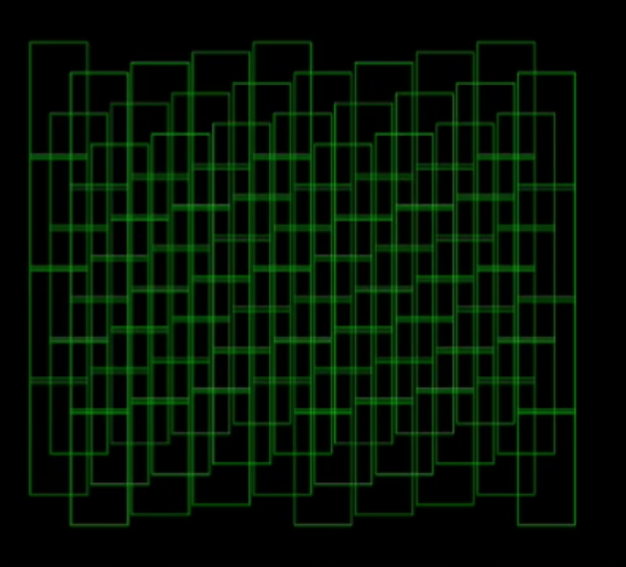
\includegraphics[width=0.5\textwidth]{image7.png}
    \caption{Minh họa Anchor Boxes}
\end{figure}

\subsection{Region Proposal Networks (RPN)}
\begin{figure}[H]
    \centering
    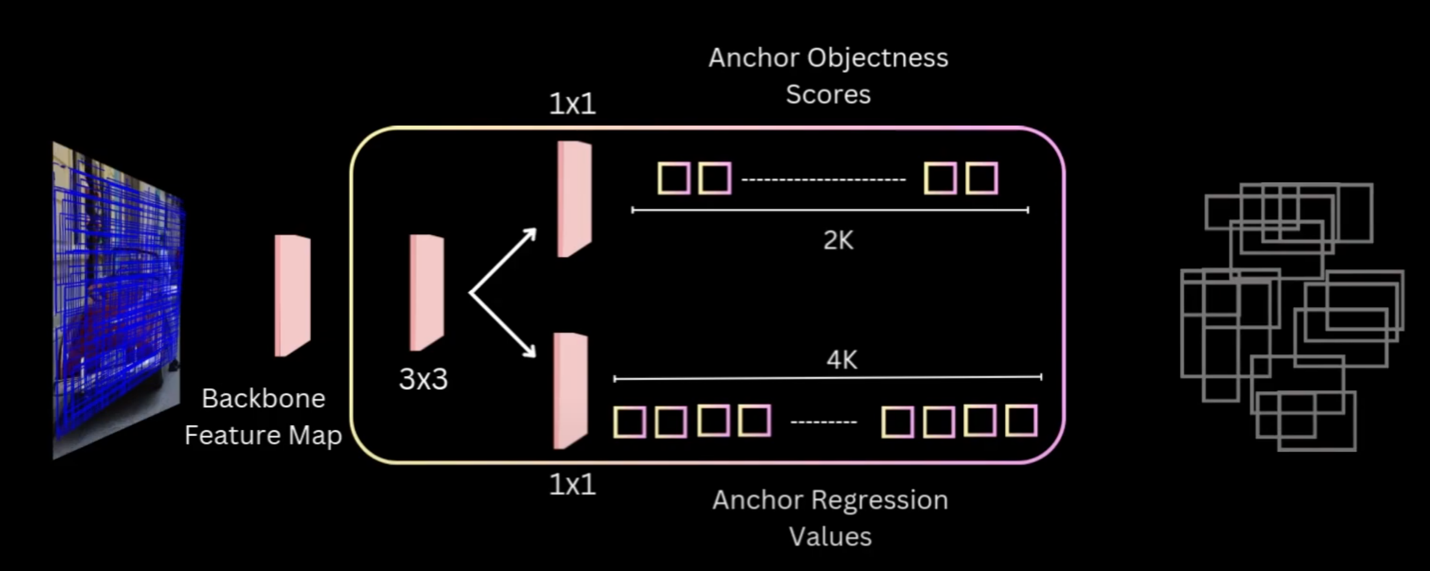
\includegraphics[width=0.8\textwidth]{image8.png}
    \caption{Region Proposal Network}
\end{figure}

\begin{itemize}
    \item Nhiệm vụ của RPN là xác định các vùng có thể chứa vật thể.
    \item Trượt một mạng CNN nhỏ 3×3 trên Feature Map. Tại mỗi vị trí của cửa sổ trượt, RPN đồng thời dự đoán nhiều vùng đề xuất dựa trên một tập hợp các anchor boxes.
    \item Tại mỗi vị trí và cho mỗi anchor box, RPN xuất ra hai tập hợp giá trị:
    \begin{itemize}
        \item Objectness Score: cho biết xác suất anchor box có chứa đối tượng hay không, thường sẽ có $2k$ giá trị, $k$ xác suất là đối tượng và $k$ xác suất là không phải đối tượng.
        \item Bounding Box Regression: điều chỉnh các kích thước của anchor box, có $4k$ giá trị vì gồm tọa độ $x, y$ và chiều rộng, chiều cao.
    \end{itemize}
    \item Giữ lại hộp tốt nhất bằng cách sử dụng Non-Maximum Suppression (NMS):
    \begin{itemize}
        \item Chọn hộp có Objectness Score lớn nhất.
        \begin{figure}[H]
            \centering
            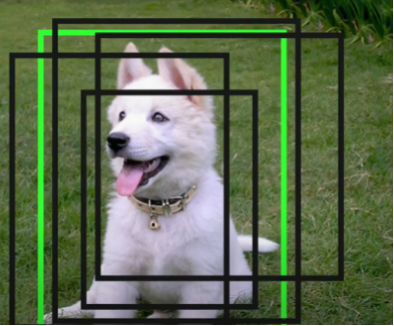
\includegraphics[width=0.5\textwidth]{image9.png}
            \caption{Chọn hộp có Objectness Score lớn nhất}
        \end{figure}
        \item Tính IoU (Intersection over Union) giữa hộp vừa chọn với các hộp còn lại.
        \begin{figure}[H]
            \begin{subfigure}{0.45\textwidth}
                \centering
                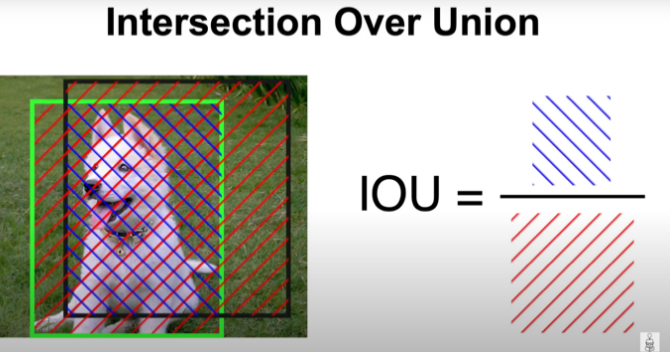
\includegraphics[width=\textwidth]{image10.png}
            \end{subfigure}
            \hfill
            \begin{subfigure}{0.45\textwidth}
                \centering
                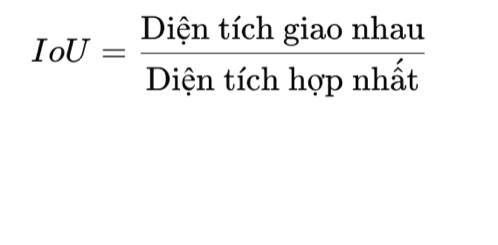
\includegraphics[width=\textwidth]{image11.png}
            \end{subfigure}
            \caption{Ví dụ tính IoU}
        \end{figure}
        \item Loại bỏ các hộp có IoU lớn hơn một ngưỡng (IoU > threshold) vì chúng được xem là trùng lặp.
        \item Ngưỡng IoU phổ biến: 0.3 - 0.5 (có thể điều chỉnh để tăng/giảm mức độ lọc).
        \item Nếu ngưỡng IoU quá cao $\rightarrow$ có thể giữ lại nhiều hộp trùng nhau.
        \item Nếu ngưỡng IoU quá thấp $\rightarrow$ có thể loại bỏ cả hộp chính xác.
    \end{itemize}
\end{itemize}

\textbf{Huấn luyện và Suy luận (Training and Inference)}
\begin{itemize}
    \item Gọi các tầng RPN (Call RPN Layers).
    \item Tạo các anchor (Generate anchors).
    \item Chuyển đổi anchor thành các đề xuất (proposal) bằng cách dự đoán biến đổi hộp (Convert anchors to Proposals using Box Transformation Prediction).
    \item Lọc các đề xuất (Filter Proposals).
\end{itemize}

\textbf{Chỉ dành cho Huấn luyện (Training Only)}
\begin{itemize}
    \item Gán các hộp Ground Truth vào các anchor (Assign Ground Truth Boxes to anchors).
    \item Tính toán nhãn và mục tiêu hồi quy cho các anchor (Compute Labels and Regression Targets for anchors).
    \item Lấy mẫu các anchor dương và âm (Sample positive and negative anchors).
    \item Tính toán Loss phân loại bằng các anchor đã lấy mẫu (Compute Classification Loss using sampled anchors).
    \item Tính toán Loss định vị bằng các anchor dương đã lấy mẫu (Compute Localization Loss using sampled positive anchors).
\end{itemize}

\subsection{Fast R-CNN detector}
Sử dụng các vùng đề xuất được tạo ra bởi RPN. Tương tự như Fast R-CNN, nó sử dụng lớp RoI Pooling để trích xuất các feature vector có kích thước cố định từ mỗi vùng đề xuất trên feature map. Sau đó, các feature vector này được đưa qua các lớp fully connected (kết nối đầy đủ) để thực hiện phân loại đối tượng (dự đoán lớp của đối tượng) và hồi quy bounding box (tinh chỉnh tọa độ của bounding box).

\begin{figure}[H]
    \centering
    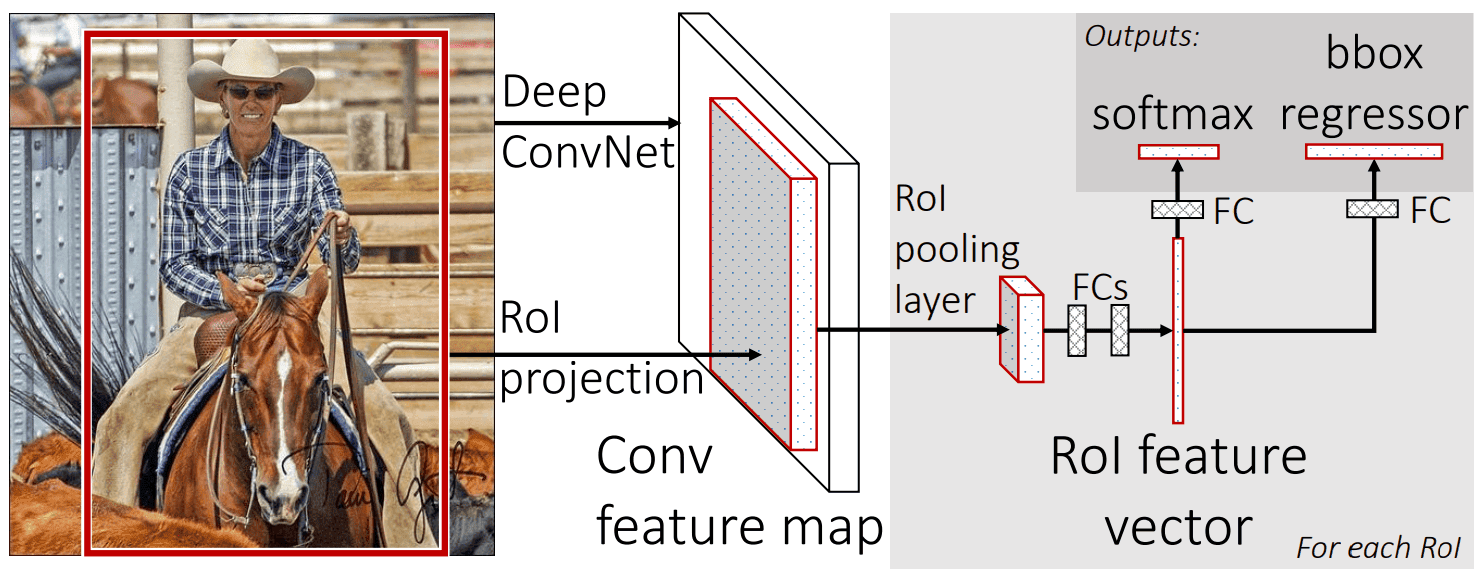
\includegraphics[width=0.8\textwidth]{image12.png}
    \caption{Kiến trúc Fast R-CNN}
\end{figure}

\textbf{RoI Pooling layer:}
\begin{itemize}
    \item Nhận đầu vào là feature map và RoI từ RPN, được biểu diễn bằng tọa độ $(x_1, y_1, x_2, y_2)$ biểu thị vùng ảnh chứa vật thể tiềm năng.
    \item Chia các RoI thành lưới $N \times N$, sau đó max pooling từng ô để tìm ra giá trị lớn nhất, ta sẽ thu được RoI luôn có kích thước cố định $N \times N$.
\end{itemize}

\begin{figure}[H]
    \centering
    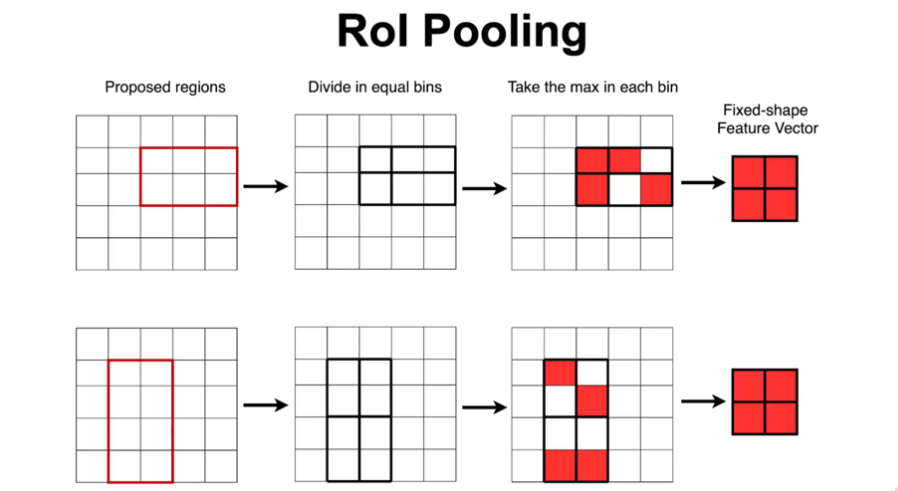
\includegraphics[width=0.5\textwidth]{image13.png}
    \caption{Ví dụ RoI Pooling}
\end{figure}

Sau khi thu được RoI feature vector, chúng ta sẽ cho vào 2 lớp FC:
\begin{itemize}
    \item Nhánh Phân loại (Classification Head): Sử dụng một lớp softmax để dự đoán điểm số lớp cho mỗi region proposal, xác định xác suất mà region proposal đó thuộc về một trong các lớp đối tượng được định nghĩa.
    \item Nhánh Hồi quy Bounding Box (Bounding Box Regression Head): Sử dụng một lớp FC khác để dự đoán các điều chỉnh (offsets) cho tọa độ của bounding box ban đầu của region proposal, nhằm tinh chỉnh vị trí và kích thước của bounding box để bao quanh đối tượng chính xác hơn.
    \item Bước cuối cùng là sử dụng Non-Maximum Suppression (NMS) để loại bỏ các hộp có thể bị trùng lặp.

\end{itemize}


\begin{tabular}{|p{0.45\textwidth}|p{0.45\textwidth}|}
\hline
\textbf{Huấn luyện (Training)} & \textbf{Suy luận (Inference)} \\ \hline
\begin{itemize}
    \item Gắn các hộp ground truth vào các đề xuất (proposals)
    \item Lấy mẫu các đề xuất trong vòng chứa ảnh
    \item Nhãn nhánh phân loại và mức tiêu chuẩn hóa các đề xuất
    \item ROI Pooling để lấy đặc trưng của đề xuất
    \item Giới hạn phân loại và hồi quy
    \item Tính toán Loss phân loại và định vị (Classification và Localization Loss)
\end{itemize} &
\begin{itemize}
    \item ROI Pooling để lấy đặc trưng của đề xuất
    \item Giới hạn phân loại và hồi quy
    \item Chuẩn hóa đề xuất thành phần dựa trên dự đoán băng cách điều chỉnh hộp (Box Transformation Prediction)
\end{itemize} \\ \hline
\end{tabular}

% Phần 3: Hàm Loss của Faster R-CNN
\section{Hàm Loss của Faster R-CNN}
Faster R-CNN sử dụng hàm mất mát (loss function) để tối ưu hóa mô hình trong quá trình huấn luyện. Hàm mất mát bao gồm:
\begin{itemize}
    \item RPN classification (binary classification, object or background).
    \item RPN regression (anchor $\rightarrow$ region proposal).
    \item Fast-RCNN classification (over $N+1$ classes, where background is also a class).
    \item Fast-RCNN bounding box regression (region proposal $\rightarrow$ ground truth bounding box).
\end{itemize}
Loss function sẽ được định nghĩa với công thức như bên dưới
\[
L(\{p_i\}, \{t_i\}) = \frac{1}{N_{\text{cls}}} \sum_i L_{\text{cls}}(p_i, p_i^*) + \lambda \frac{1}{N_{\text{reg}}} \sum_i p_i^* L_{\text{reg}}(t_i, t_i^*)
\]
\begin{itemize}
    \item $i$ là index của anchor trong 1 mini-batch.
    \item $p_i$ là xác suất dự đoán cho anchor tại index thứ $i$ là 1 đối tượng.
    \item $L_{cls}$ với RPN là binary cross-entropy để xác định anchor có chứa đối tượng (object) hay không.
    \item $L_{cls}$ với Fast-RCNN tại phần cuối của mô hình là Multi-class cross-entropy loss với $(N + 1)$ classes.
    \item $L_{reg}$ là loss tính cho bounding box regression. Loss cho bounding box regression chỉ được tính khi anchor là positive:
\end{itemize}
\[
L_{1,smooth} = 
\begin{cases} 
|x| & \text{if } |x| > a \\
\frac{1}{a} x^2 & \text{if } |x| \leq a
\end{cases}
\]

% Phần 4: Input đầu vào và cách train mô hình Faster R-CNN
\section{Input đầu vào và cách train mô hình Faster R-CNN}
Dữ liệu đầu vào gồm:
\begin{itemize}
    \item Ảnh gốc: Kích thước bất kỳ.
    \item Ground Truth Bounding Boxes: Hộp giới hạn chứa vật thể, định dạng $(x, y, w, h, c)$ với:
    \begin{itemize}
        \item $x, y$: Tọa độ tâm hộp.
        \item $w, h$: Chiều rộng và chiều cao.
        \item $c$: Nhãn vật thể.
    \end{itemize}
\end{itemize}

Ví dụ:
\begin{verbatim}
{
    "id": 383,
    "image_id": 108,
    "category_id": 1,
    "bbox": [218, 390, 20, 38],
    "area": 760,
    "segmentation": [],
    "iscrowd": 0
}
\end{verbatim}

Quá trình train bao gồm:
\begin{itemize}
    \item Resize ảnh về kích thước chuẩn.
    \item Normalize giá trị pixel về [0,1] hoặc [-1,1].
    \item Tạo các Anchors với nhiều tỷ lệ khác nhau cho RPN.
    \item Ảnh qua Backbone CNN (ResNet/VGG) $\rightarrow$ tạo Feature Map.
    \item Dự đoán hộp giới hạn tiềm năng.
    \item So sánh với Ground Truth để tối ưu bằng RPN Loss.
    \item Các hộp từ RPN được chuẩn hóa bằng RoI Pooling.
    \item Dự đoán nhãn và tinh chỉnh hộp bằng Softmax \& Bounding Box Regression Loss.
    \item Sử dụng Backpropagation + Gradient Descent để tối ưu mô hình.
    \item Loss function kết hợp Classification Loss + Bounding Box Loss + RPN Loss.
\end{itemize}

% Phần 5: Đánh giá độ chính xác của mô hình
\section{Đánh giá độ chính xác của mô hình}

\subsection{Đánh giá IoU}
IoU là thước đo để đánh giá mức độ trùng khớp giữa hộp dự đoán và hộp thực tế (ground truth). Công thức tính:
\[
\text{IoU} = \frac{\text{Area of Overlap}}{\text{Area of Union}}
\]
Nếu IoU $\geq$ 0.5, dự đoán được xem là đúng (True Positive - TP). \\
Nếu IoU < 0.5, dự đoán là sai (False Positive - FP).

\subsection{Precision, Recall và F1-Score}
Dựa vào IoU, ta xác định được các giá trị:
\begin{itemize}
    \item True Positive (TP): Hộp dự đoán đúng (IoU $\geq$ 0.5).
    \item False Positive (FP): Hộp dự đoán sai (IoU < 0.5).
    \item False Negative (FN): Hộp thực tế có nhưng không được dự đoán.
\end{itemize}

Precision:
\[
\text{Precision} = \frac{\text{TP}}{\text{TP} + \text{FP}}
\]
Xác suất một hộp dự đoán thực sự chứa vật thể. Precision cao khi ít hộp bị phát hiện sai.

Recall:
\[
\text{Recall} = \frac{\text{TP}}{\text{TP} + \text{FN}}
\]
Recall cao khi mô hình không bỏ sót vật thể. Tỉ lệ số vật thể thực tế được phát hiện.

F1-Score: cân bằng giữa recall và precision
\[
\text{F1} = 2 \times \frac{\text{Precision} \times \text{Recall}}{\text{Precision} + \text{Recall}}
\]

\subsection{Mean Average Precision (mAP)}
mAP là thước đo phổ biến để đánh giá mô hình nhận diện vật thể.
\begin{itemize}
    \item Với mỗi lớp vật thể, ta vẽ Precision-Recall Curve.
    \item Tính diện tích dưới đường cong để có Average Precision (AP).
    \item mAP là trung bình của tất cả các AP trên các lớp vật thể.
\end{itemize}
\[
\text{mAP} = \frac{1}{N} \sum_{i=1}^{N} \text{AP}_i
\]
$N$ là số lớp trong tập dữ liệu.
\begin{itemize}
    \item mAP > 0.7: Mô hình rất tốt.
    \item mAP từ 0.5 - 0.7: Mô hình hoạt động khá ổn.
    \item mAP < 0.5: Cần cải thiện mô hình.
\end{itemize}

% Phần 6: Cách cải thiện mô hình
\section{Cách cải thiện mô hình}
\begin{itemize}
    \item Tăng số lượng dữ liệu huấn luyện, giảm overfitting.
    \item Tăng cường dữ liệu, giúp nhận diện tốt hơn trong các điều kiện khác nhau.
    \item Điều chỉnh kiến trúc mô hình:
    \begin{itemize}
        \item Sử dụng các lớp tích chập phức tạp hơn.
        \item RPN tăng thêm số vùng đề xuất tránh mất vật thể.
        \item Điều chỉnh anchor box phù hợp.
    \end{itemize}
    \item Tối ưu hóa huấn luyện:
    \begin{itemize}
        \item Bắt đầu với learning rate lớn rồi giảm dần theo từng epoch.
        \item Dừng huấn luyện sớm nếu loss không giảm để tránh overfitting.
        \item Dùng Dropout, Weight Decay để giúp mô hình tổng quát tốt hơn.
    \end{itemize}
\end{itemize}

% Phần 7: Kết quả của mô hình với nhận diện có mũ hay không có mũ
\section{Kết quả của mô hình với nhận diện có mũ hay không có mũ}
\begin{itemize}
    \item Dataset khoảng 4000 ảnh.
\end{itemize}

\begin{figure}[H]
    \centering
    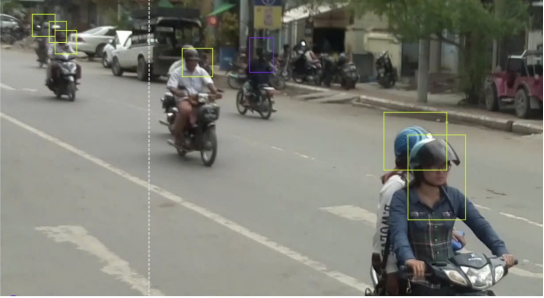
\includegraphics[width=0.8\textwidth]{image14.png}
    \caption{Dataset minh họa}
\end{figure}

\begin{itemize}
    \item Training với 20 epoch trong vòng 3 giờ.
    \item Đánh giá mô hình với kết quả dự đoán là:
    \begin{itemize}
        \item Precision: 0.8950
        \item Recall: 0.8971
        \item F1: 0.8960
        \item mAP 0.5: 0.4776
    \end{itemize}
\end{itemize}

\begin{figure}[H]
    \centering
    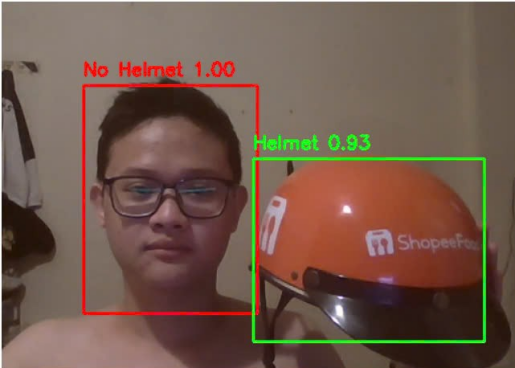
\includegraphics[width=0.8\textwidth]{image15.png}
    \caption{Kết quả đánh giá mô hình}
\end{figure}

Các hạn chế của mô hình Faster-RCNN:
\begin{itemize}
    \item Nhận diện realtime không tốt.
    \item Mô hình phức tạp cần sự hiểu biết cao.
    \item Tốn nhiều tài nguyên như GPU.
    \item Cần số lượng dataset lớn và rõ.
\end{itemize}

Một số nhận diện lỗi của mô hình:
\begin{figure}[H]
    \centering
    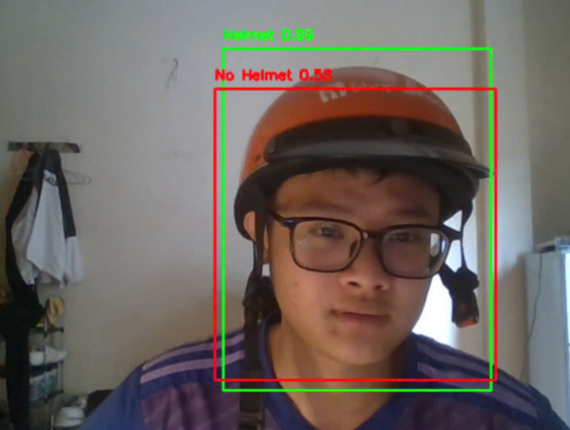
\includegraphics[width=0.8\textwidth]{image16.png}
    \caption{Ví dụ nhận diện lỗi}
\end{figure}

% Phần 8: So sánh mô hình với Yolo-v12
\section{So sánh mô hình với Yolo-v12}
Khác với các mô hình truyền thống như Faster R-CNN hoạt động theo hai giai đoạn, YOLO là mô hình phát hiện một giai đoạn (one-stage), tức là mô hình trực tiếp dự đoán các bounding box và nhãn lớp trong một lần xử lý duy nhất. Điều này giúp YOLO có tốc độ rất nhanh, phù hợp với các ứng dụng yêu cầu xử lý thời gian thực (real-time).

\begin{figure}[H]
    \begin{subfigure}{0.45\textwidth}
        \centering
        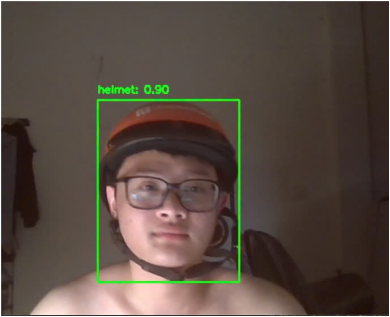
\includegraphics[width=\textwidth]{image17.png}
    \end{subfigure}
    \hfill
    \begin{subfigure}{0.45\textwidth}
        \centering
        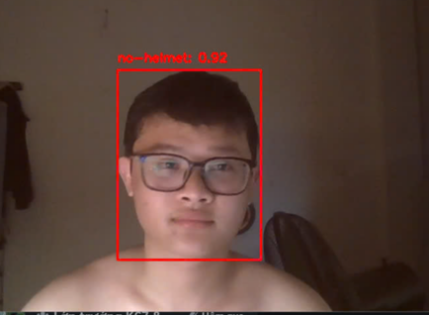
\includegraphics[width=\textwidth]{image18.png}
    \end{subfigure}
    \caption{Ví dụ kết quả Faster R-CNN và YOLO}
\end{figure}

\begin{center}
\begin{tabular}{|l|l|l|}
\hline
\textbf{Tiêu chí} & \textbf{Faster R-CNN} & \textbf{YOLO} \\ \hline
Precision         & 0.8950               & 0.87795       \\ \hline
Recall            & 0.8971               & 0.80614       \\ \hline
F1                & 0.8960               & 0.84022       \\ \hline
mAP 0.5           & 0.4776               & 0.87686       \\ \hline
mAP [0.5:0.95]    & 0.2161               & 0.58504       \\ \hline
FPS               & 5-7                  & 30-60         \\ \hline
Nhận diện vật thể nhỏ & Tốt                  & Hạn chế nếu không tối ưu \\ \hline
Tải nghiệm cần    & Cao                  & Thấp          \\ \hline
Độ phức tạp       & Cao                  & Thấp          \\ \hline
Mục đích          & Phù hợp với tính chất offline, phân tích & Phù hợp với ứng dụng thời gian thực \\ \hline
\end{tabular}
\end{center}

% Phần 9: Các kết quả trong quá trình huấn luyện và triển khai mô hình với Yolo
\section{Các kết quả trong quá trình huấn luyện và triển khai mô hình với Yolo}
\begin{figure}[h]
    \centering
    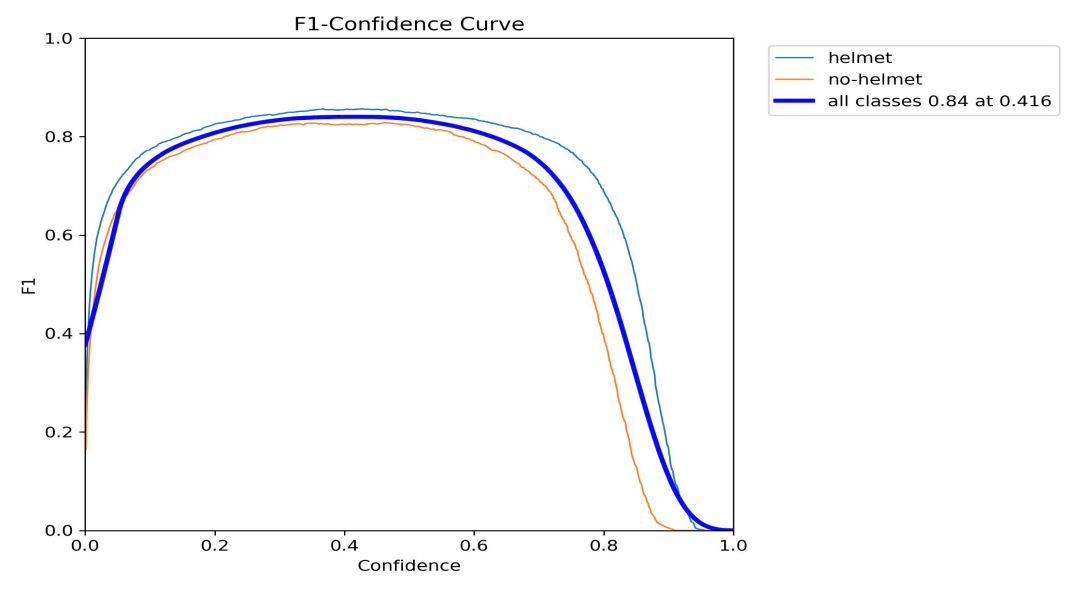
\includegraphics[width=0.8\textwidth]{image19.png}
    \caption{Biểu đồ huấn luyện YOLO}
\end{figure}

\begin{figure}[h]
    \centering
    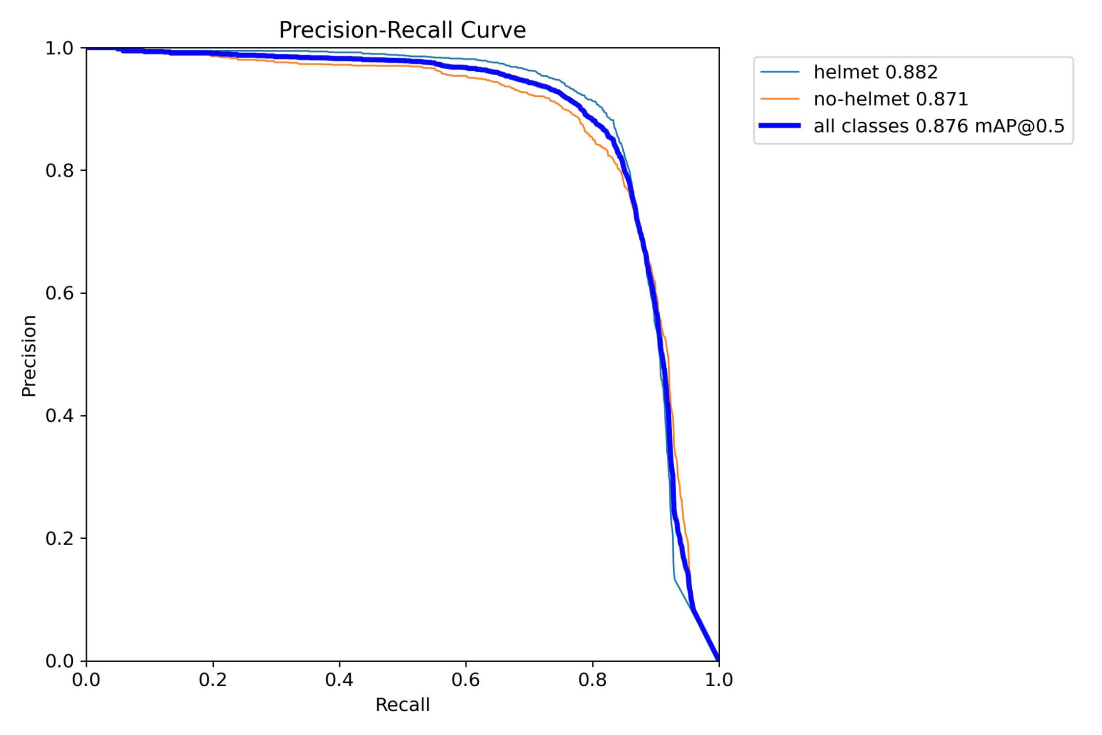
\includegraphics[width=0.8\textwidth]{image20.png}
    \caption{Biểu đồ giá trị dự đoán YOLO}
\end{figure}

\begin{figure}[h]
    \centering
    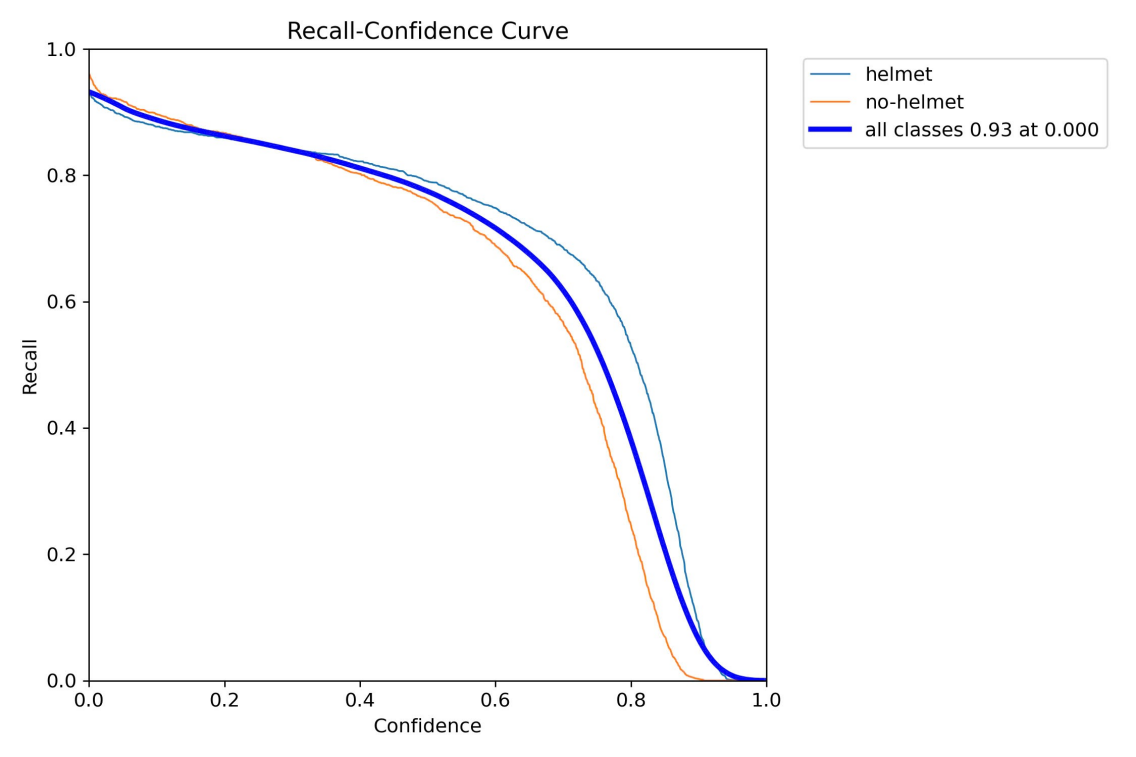
\includegraphics[width=0.8\textwidth]{image21.png}
    \caption{Kết quả triển khai YOLO}
\end{figure}

\begin{figure}[h]
    \centering
    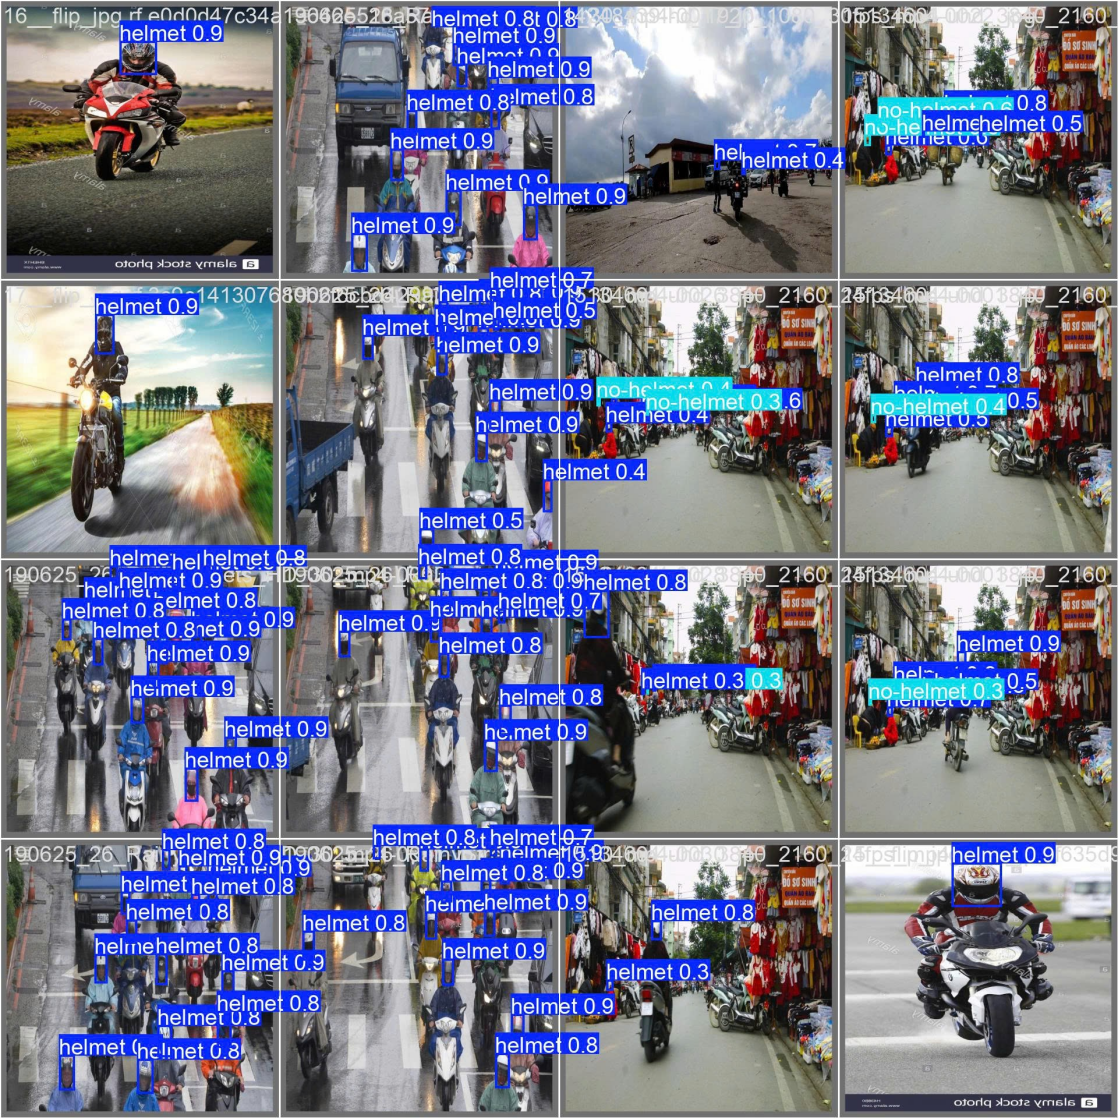
\includegraphics[width=0.8\textwidth]{image22.png}
    \caption{Kết quả triển khai YOLO}
\end{figure}

\end{document}